\documentclass[a4paper, 11pt, onecolumn, compsoc, twoside]{IEEEtran}
\usepackage{xcolor}
\usepackage{listings}			% Used to include VHDL-code and fragments
\lstset{basicstyle=\ttfamily,
  showstringspaces=false,
  commentstyle=\color{red},
  keywordstyle=\bf\color{blue},
  tabsize=4
}
\renewcommand{\lstlistingname}{Script}% Listing -> Script
\usepackage[english]{babel}		% English hyphenation patterns and english names 
\usepackage{pslatex}			% Times, helvetica and courier
\usepackage[T1]{fontenc}		% Nicer font-encoding
\usepackage[hidelinks]{hyperref}% Gives clickable references in pdf-file
\usepackage{graphicx}			% Used to include .pdf, .jpg and .png-files
\usepackage{tabularx}			% Used for evenly spread tables
\usepackage{eso-pic}			% Absolute positioning, used for lines-to-track appendix and front- and backpage
\usepackage{datetime}			% Used for some data-references
\usepackage[font=small,format=plain,labelfont=bf,up,textfont=up]{caption}	% Nicer captions
\usepackage{subcaption}
\usepackage{nonfloat}			% Captions for non-floating figures and tables
\usepackage{nextpage}			% Advanced nextpage commands
\usepackage{keystroke}			% "real" keys
%\usepackage[nottoc]{tocbibind}		% Include Bibliography in ToC
\usepackage{multirow}			% Span text over multiple rows
\usepackage{verbatim}			% For comment-environment
\usepackage[left=3.5cm, right=2.5cm]{geometry}
\usepackage[section]{placeins}  %zorgt ervoor dat floats niet onder een andere section komen, want dat is vervelend!
\usepackage{lmodern}
\usepackage{amsmath}
%\usepackage[nottoc,notlot,notlof]{tocbibind}
\usepackage{ntheorem}
%\usepackage[retainorgcmds]{IEEEtrantools}
\usepackage{a4wide}
\usepackage{gensymb}
\usepackage{cite}
\usepackage{amsfonts}
\usepackage{longtable}
\usepackage{soul}
\usepackage{import}
\usepackage{placeins} %use \FloatBarrier to prevent figs/tabulars into other (sub)section
\usepackage{cleveref}  % the Smart Reference, just use \cref{name}.
\usepackage{enumitem, hyperref} % om te kunnen refereren naar het programma van eisen
\makeatletter
\def\namedlabel#1#2{\begingroup
    #2%
    \def\@currentlabel{#2}%
    \phantomsection\label{#1}\endgroup
}
\makeatother
%\setlength\parindent{0pt}

%%%%%%%%%%%%%%%%%%%%%%%%%%%%%%%%%%%%%%%%%%%%%%%%%%%%%%%%%%%%%%%%%%%%%%
% Settings
%%%%%%%%%%%%%%%%%%%%%%%%%%%%%%%%%%%%%%%%%%%%%%%%%%%%%%%%%%%%%%%%%%%%%%

% Settings for hyperref-package
\hypersetup{	colorlinks	= false,		%
		pdfborder	= 0 0 0}		%

% Settings for listings-package
\lstset{	numbers		= left,			%
		numberstyle	= \tiny,		%
		numbersep	= 5pt,			%
		language	= VHDL,			%
		breaklines	= true,			%
		showspaces	= false,		%
		showstringspaces= false}

%%%%%%%%%%%%%%%%%%%%%%%%%%%%%%%%%%%%%%%%%%%%%%%%%%%%%%%%%%%%%%%%%%%%%%



\begin{document}

	\newcounter{tempcounter}	% For temporarily breaking enumerate-environments

	\pagestyle{empty}		% To prevent pagenumber on backside of titlepage
	% Frontpage with image
\AddToShipoutPicture*{
	\setlength{\unitlength}{1cm}
	\put( 0,  0){\includegraphics{images/TUDelft_border1}}	%PDF version 1.5 preferred
	\put( 1, 13){\color{cyan}\linethickness{2cm}\line(0,1){7}}
	\put( 1, 13.5){\rotatebox{90}{\color{white}\large\textsf{Delft University of Technology}}}
	\put( 2, 23){\color{black}\linethickness{6cm}\line(1,0){15.5}}
	\put( 3, 25){\color{white}{\large{EE3L11}}}
	\put( 3, 24){\color{white}{\Huge{Project SUNRISE:}}}
	\put( 3, 23){\color{white}{\Huge{Control for Solar Powered e-bike}}}
	\put( 3, 22){\color{white}{\Huge{Charging Station}}}
	\put( 3, 21){\color{white}{\large{Group D, Team ODROID}}}
%	\put( 4, 8){\includegraphics[width=11cm]{images/Matlab_graph4}}
%	\put( 3,  7.0){\large{BAP Team D, Groep ODROID}}
	\put( 3, 6.5){\large{T.B. Hosman, 4275691}}
	\put( 3,  6.0){\large{Job van Staveren, 4317386}}
	\put( 3,  5){\large{\today}}
	\put( 3,  4.5){\large{Version 1.0}}
}
~
\clearpage



%	\input{versieoverzicht}
	\begin{abstract}
%\setlength\parindent{0pt}
In the summer of 2016, a solar-powered charging station for e-bikes (both wired and wireless) and e-scooters will be built on the campus of Delft University of Technology. This station is also meant to provide a testing facility for future projects. The station has a number of systems that generate data: the power electronics (including the solar panels, batteries and grid-connection), a weather station, solar panel temperature sensors and the connected vehicles.\\

The SUNRISE (Smart Unified Networking Rig for an Integrated Solar E-bike charger) project is a BSc final project that should log and display all this data through an administrator page, a website and a local display. It should also be able to manage e-bike users that would like to connect to the station.\\

Team ODROID was responsible for the local data management and charger control. The team managed to fetch all necessary data from the power electronics, temperature probes and weather station with C-code running on an ODROID C1+. Furthermore, the developed system was designed from the start to be robust (since it will be running 24/7) and has been thoroughly tested for possible malfunctions. The system has also been made resistant against power and internet outages. Moreover, the system can register e-bike cable connections, which it uses to fully control the chargers. It also provides data necessary to display system information on a local display. Finally, the entire system is remotely controllable through a remote desktop.
\end{abstract}
 
    
	\pagestyle{headings}


	\clearpage
	\tableofcontents
	\clearpage
    
    
%%%%%%%%%%%%%%%%%%%%%%%%%%%%%%%%%%%%%%%%%%%%%%%%%%%%%%%%%%%%%%%%%%%%%%
% 				The Input Files for each Section here:
%%%%%%%%%%%%%%%%%%%%%%%%%%%%%%%%%%%%%%%%%%%%%%%%%%%%%%%%%%%%%%%%%%%%%%
	\section{Introduction}\label{sec:introduction}
This project is part of a solar-powered e-bike charging station that will be built on the campus of Delft University of Technology. This station consists of power electronics to manage power between the solar panels, the station batteries, the grid and all the connected vehicles. The station is able to charge e-bikes both wired and wirelessly, as well as e-scooters. The station also has a weather station to monitor the outside climate. Furthermore, the system has a number of temperature sensors to monitor the temperature levels of the solar panels. A concept of the station can be found in \Cref{fig:station_concept}.

\begin{figure}[!ht]
  \centering
    \includegraphics[width=0.6\textwidth]{images/charging_station.png}
      \caption{Concept of the solar powered e-bike charging station \cite{feasibility_study}}\label{fig:station_concept}
\end{figure}

The SUNRISE project (Smart Unified Networking Rig for an Integrated Solar E-bike charger) was proposed as a final BSc project. The result of this project should manage the data generated by the power electronics, weather station and temperature probes through a local mini computer and log the information on a TU Delft server. This mini computer should also control a local display that shows live information about the system. SUNRISE should also be able to handle requests of registered users that want to charge their vehicle at the station. The input is processed through a webpage hosted by the university, which should trigger the station to turn on one of the chargers. The webpage will then comunicate to the user what charger to use, after which the user will be able to monitor the state of their battery through the webpage. Finally, the SUNRISE project should have an administrator dashboard to show the status and data of the system, and a media webpage that will display some basic information to the media. An overview of the entire system can be found in \Cref{fig:project_overview}.

\begin{figure}[!ht]
  \centering
    \includegraphics[width=1.0\textwidth]{images/project_overview.pdf}
      \caption{An overall view of the entire SUNRISE system}\label{fig:project_overview}
\end{figure}
	\subsection{Problem definition}
Team ODROID of the SUNRISE project group will focus on the local mini computer, which does all the data acquisition, as well as the control of the local display. It should also be able to control the chargers and register any charger that gets disconnected. It is important that there is a focus on robustness, because the system should run 24/7. A more detailed description can be found in \Cref{sec:requirements}.
	\subsection{State-of-the-art analysis}
In the last few years some work has already been done regarding the project as described in \Cref{sec:introduction}. As a consequence, the work to be done for this design can partially be built on these results.\\

A major contribution was made in the development of C-code that is able to perform a few conceptual tasks \cite{report_pavel}. For example, this code is able to establish a connection with some devices connected to the ODROID and can read a register from those devices. However, it was not tested with all devices (e.g. temperature sensors) and it was not known what registers were read. The code also contains some functions to send data to the server and database, as well as a function to control the local display at the charging station. Beside the code, the report contained general information about the devices and C-code \cite{report_pavel}. It also contains a short description of the functions and protocols being used.\\

The Victron power electronics system, the weather station and the temperature probes all communicate using Modbus. For C there is a library called \textit{libmodbus} \cite{libmodbus} that can be used to ease communication. By using this library, the communication can be done at a much higher level using the standard Modbus communication routines. Moreover, this library contains support for both Modbus RTU and Modbus TCP which are needed to read the registers from the Victron power electronics system (Modbus TCP) and the weather station and temperature probes (Modbus RTU).\\

Another C library that is available for working with the ODROID is the \textit{WiringPi} library \cite{WiringPi}. This library is used to easily assign logic values to the GPIO pins of the ODROID.\\



% cite naar zowel code als report van Pavel?
	\subsection{Overview}
This thesis will start off with the general requirements of the system in the programme of requirements (\Cref{sec:requirements}). It will then give a general description of all the code modules, as well as the choices made regarding these modules (\Cref{sec:design}). This section will begin with a code overview (\Cref{sec:code_overview}) after which it will go into more detail regarding the weather station (\Cref{sec:weather_station}), Victron power management system (\Cref{sec:Victron}), solar panel temperature sensors (\Cref{sec:temp_sensors}), chargers (\Cref{sec:chargers}), local display (\Cref{sec:display}) and bash scripts (\Cref{sec:bash}). The thesis will then go over the validation tests and robustness of the system in the results (\Cref{sec:results}) after which they will be discussed (\Cref{sec:discussion}). The thesis will conclude in \Cref{sec:conclusions}, in which there will also be some future recommendations (\Cref{sec:future}).
        \clearpage 	   
	\section{Programme of requirements}\label{sec:requirements}
In the high-level user and admin interface, status information about the chargers and power electronics is needed, as well as general information about the weather. To obtain this information, the ODROID must read this data from the corresponding components in the system. 
This data is then sent to the server from which it is eventually displayed in the user/admin interface. Another main task of the ODROID is to turn the chargers for the electric vehicles on and off. Finally, there is an external display placed in the charging station which shows some general information about the weather, as well as availability of charging points.

\subsection{Functional Requirements}
%Volgens handleiding moet PoR genummerd worden

Functional requirements determine what the design must be able to do and which functionalities it must have. Based on the problem definition the following functional requirements are determined.\\
The design must be able to:
\begin{itemize} 
\item[\namedlabel{eis:1.1}{[1.1]}] Read the data from the weather station.
\item[\namedlabel{eis:1.2}{[1.2]}] Read the data from the Victron power electronics system.
\item[\namedlabel{eis:1.3}{[1.3]}] Read the temperatures from the temperature probes.
\item[\namedlabel{eis:1.4}{[1.4]}] Control the local display at the e-bike charging station.
\item[\namedlabel{eis:1.5}{[1.5]}] Show general information about weather and availability of the charging points.
\item[\namedlabel{eis:1.6}{[1.6]}] Turn the chargers on and off based on server and sensor information.
\end{itemize}

\subsection{System requirements}
Requirements that are not functional but are important for the utilisation are the system requirements \cite{baphandleiding}. In this case these requirements merely put constraints on the software and ODROID once they are installed in the e-bike charging station.\\
The system must:
\begin{itemize}
\item[\namedlabel{eis:2.1}{[2.1]}] Be accessible via a remote desktop.
\item[\namedlabel{eis:2.2}{[2.2]}] Be able to recover itself after a power or internet failure.
\item[\namedlabel{eis:2.3}{[2.3]}] Run the software 24 hours a day, 7 days a week.
\end{itemize}


\subsection{General Conditions}
The general conditions are determined by the framework in which this project is carried out. Other general condition are a result of constraints from the components used for this project. The general conditions are:
\begin{itemize}
\item[\namedlabel{eis:3.1}{[3.1]}] The system has to be controlled by a minicomputer (i.e. Raspberry Pi or ODROID).
\item[\namedlabel{eis:3.2}{[3.2]}] Connected devices are bound to a maximum polling rate.
\item[\namedlabel{eis:3.3}{[3.3]}] The sofware for the mini computer has to be written in C.
\item[\namedlabel{eis:3.4}{[3.4]}] The charging station can facilitate four e-bikes, one electric scooter and one electric vehicle that can be charged wirelessly.
\end{itemize}

% Hier moet misschien nog een mooi verhaaltje achter
		\clearpage    	
	\section{Design and implementation}\label{sec:design}
This section will go through all the designed modules used in the system. The mini computer that is used will be the ODROID C1+ \ref{eis:3.1}, which was chosen due to its availability within the DC\&S research group. The ODROID C1+ will now be referred to as ODROID.
	\subsection{Code overview}\label{sec:code_overview}
The C-code \ref{eis:3.3} that will manage all the data on the ODROID consists of several elements. An overview of how these elements and their data are managed can be found in \Cref{fig:code_overview}.\\

\begin{figure}[!ht]
  \centering
    \includegraphics[width=1.0\textwidth]{images/ODROID_code_overview.pdf}
      \caption{An overview of the C code}\label{fig:code_overview}
\end{figure}

The entire program is built around a variable \verb|j| that keeps track of time by incrementing every 1.5 seconds. This variable resets to zero every time it is reaches 400, creating a loop that restarts every 10 minutes.\\

The ODROID will decide what data to handle based on this variable. For every j, the ODROID will fetch the charger states from the server and set the chargers using the \verb|setChargers()| function. Every 5 minutes (when \verb|j| equals 100 or 300), data from the weather station is fetched and sent to the server (\verb|weatherDisplay(1)|). Every 15 seconds (when \verb|j| is a multiple of 10), data will also be fetched from the weather station, but only to refresh the local display (\verb|weatherDisplay(0)|). To prevent this event from causing two data fetches to the weather station, it is only run if it does not conflict with \verb|weatherDisplay(1)| (by using \verb|else if|). Note that \verb|weatherDisplay(0)| does not increment \verb|j|, so it is possible that it runs together (before) the functions starting at \verb|j| equal to 400 or 200.\\

Every 10 minutes (when \verb|j| equals 200), data from the temperature probes is read. This data is also sent to the server. A similar loop is also run every 10 minutes (when \verb|j| equals 400) which will read the Victron data. This loop will be run 3 times because there are three seperate chunks of data that will be read (further explained in \Cref{sec:Victron}). Every chunk of data is seperately sent to the server.\\
	\subsection{Weather station}\label{sec:weather_station}
One of the devices that is connected to the ODROID is the Lufft WS503-UMB weather station \cite{weatherstation_registers}. It is connected to an adapter that converts the Modbus RTU connection to an USB that can be connected to the ODROID (See \Cref{fig:weather_station_connection}). This station is capable of measuring air pressure, relative humidity, solar radiation, air pressure, wind direction and wind speed. The data that this weather station processes is collected \ref{eis:1.1} and used to display local weather information to both the user \ref{eis:1.6} and the administrator. It could also be used to add functionality, such as disabling charging when the outside temperature is too low \cite{battery_temperature} or checking if the solar panels are functioning by comparing output power to solar radiation.\\

\begin{figure}[!ht]
  \centering
    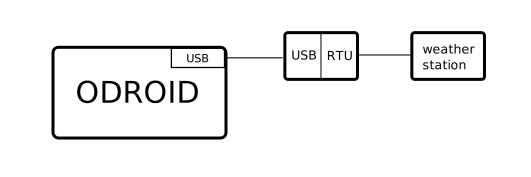
\includegraphics[width=0.6\textwidth]{images/ODROID_weather_station.pdf}
      \caption{The connection of the weather station}\label{fig:weather_station_connection}
\end{figure}

The polling of the weather stations registers is set to roughly every 15 seconds. Although the maximum polling rate \ref{eis:3.2} is technically possible of going down to 10 seconds \cite{weatherstation_polling_rate}, it was decided that 15 seconds was more than enough to refresh the local display.\\

\subsubsection{Register data}\label{sec:weather_station_register_data}
The weather station that is used has a total of 121 registers that can be read. Most registers, however, are merely values derived from another (e.g. US units). It is therefore decided that it is unnecessary to read all the data that can be found in the registers. The registers that are read by the ODROID are:
\begin{itemize}
\item Sensor statusses (registers 2 - 6)
\item Relative humidity as percentage (register 13)
\item Relative air pressure in hPa (register 17)
\item Wind direction in degrees (register 18)
\item Global radiation in W/m$^2$ (register 30)
\item Air temperature in Celcius (register 34)
\item Wind speed in m/s (register 45)\\
\end{itemize}

All data will be sent as a \verb|double| array to the server. All data is decoded by casting and scaling functions before sending to the sever, this is done similar to the Victron data (see \Cref{sec:casting} and \ref{sec:scaling}). Sensor status data is not sent decoded when cast to a \verb|double|, however it is easier to send as a \verb|double| because it can be placed in the array to be sent. The actual decoding (see \Cref{sensor_status_list}) is done server-side. This method causes redundant sensor data (statusses with a strikethrough in \Cref{sensor_status_list}) to be sent, but this is hardly of any impact on the server.

\begin{table}
\centering
\caption{Sensor status coding}
\begin{tabular}{|l|l|l|l|l|}
\hline
\textbf{Register} & \multicolumn{2}{c|}{\textbf{High byte}}  & \multicolumn{2}{c|}{\textbf{Low byte}} \\ \hline
  & \textbf{High half-byte} & \textbf{Low half-byte} & \textbf{High half-byte} & \textbf{Low half-byte} \\ \hline
2 & Air temperature buffer & Air temperature & \st{Dew point buffer} & \st{Dew point} \\ \hline
3 & Rel. humidity buffer & Rel. humidity & \st{Abs. humidity buffer} & \st{Abs. humidity} \\ \hline
4 & \st{Mixing ratio buffer} & \st{Mixing ratio} & Air press. buffer & Air pressure \\ \hline
5 & Wind & Wind buffer & \st{Precipitation} & \st{Compass} \\ \hline
6 & Global radiation buffer & Global radiation & \st{Leaf wetness buffer} & \st{Leaf wetness} \\ \hline
\end{tabular}
\label{sensor_status_list}
\end{table}

\subsubsection{Read function}
The \verb|readWeatherStation| function was made to read registers from the weather station. It was designed to be flexible, so it is easy to change what registers to read. The first argument of the function, \verb|registersToRead[]| is an integer array of a flexible length, where an element corresponds to the register number that has to be read. The second argument is the length of this array. An example of calling this function can be found in Script \ref{readWeatherStation}. The registers in this example correspond to the registers mentioned in \Cref{sec:weather_station_register_data}. Note that \verb|readWeatherStation| writes to an array that is initialized at the start of the program and globally writeable (further explained in \Cref{sec:malloc}).\\

\scriptsize
\begin{lstlisting}[language=C,caption={Read function},label={readWeatherStation}]
	int registersToRead[] = {2, 3, 4, 5, 6, 34, 39, 13, 45, 30, 17, 18};
	int length = sizeof(registersToRead)/sizeof(int);
	if (readWeatherStation(registersToRead, length)){
		...
	}
\end{lstlisting}
\normalsize

\subsubsection{Robustness}\label{sec:weather_robustness}
A couple of checks are done in \verb|readWeatherStation| to ensure that the system can run 24/7 \ref{eis:2.3}. This is done by returning zero whenever a check fails. The function that handles the data (see \Cref{sec:code_overview}) will then check if a zero was returned. Whenever this happens, it will bypass updating the local display and the sending of data to the server. This is done in the \verb|if|-statement of Script \ref{readWeatherStation}. These checks are inspired by the previously designed code \cite{report_pavel}.\\

One of the checks that is executed every call of the function is the code found in Script \ref{rc_check}. In this statement, \verb|rc| (the length of the array that is received from the weather station) is compared to \verb|numberOfRegisters| (the number of registers that is requested). This ensures that all data is received, and that the modbus connection was not lost halfway transmitting. Either way, necessary information is printed and the modbus connection is closed. Memory is freed if necessary.\\

\scriptsize
\begin{lstlisting}[language=C,caption={Comparing rc to numberOfRegisters},label={rc_check}]
if(rc==numberOfRegisters)
{
    for (i=0; i<tabs; i++)
    {
        printf("OK, value %f \n",weatherFinalValues[i]);
    }
    modbus_close(ctx);
    modbus_free(ctx);
    return 1; //return success
}
else
{
    printf("FAILED (nb points %d) \n",rc);
    modbus_close(ctx);
    modbus_free(ctx);
    return 0; //return failure
}
\end{lstlisting}
\normalsize

Another check can be found in Script \ref{check_modbus_connection}. This piece of code checks if the connection with the weather station has been successful.\\

\scriptsize
\begin{lstlisting}[language=C,caption={Checking if a connection can be established with the weather station},label={check_modbus_connection}]
	if (modbus_connect(ctx) == -1){
		fprintf(stderr,"Connection failed: %s\n",modbus_strerror(errno));
		modbus_free(ctx);
		return 0;
	}
\end{lstlisting}
\normalsize

Finally, Script \ref{check_register_input} checks if all requested registers are available. This should generally not happen if the programmer knows what he is doing, so technically only the \verb|stderr| notification is needed. However, a return value of zero is added to ensure that the rest of the code can be tested even when something went wrong in the weather station. Note that this piece of code also includes the line of code where filtering and scaling is done (line 12). Scaling done in this line is further explained in \Cref{sec:scaling}.

\scriptsize
\begin{lstlisting}[language=C,caption={Checking if the requested registers are available},label={check_register_input}]
    for (i=0; i<tabs; i++)
    {
        // requested register exceeds range of registers that is available
        if (registersToRead[i] > (nb_points-1))
        {
            fprintf(stderr,"Requested %d weatherstation register unavailable\n", registersToRead[i]);
            modbus_close(ctx);
            modbus_free(ctx);
            return 0; //return failure
        }
        //filter and scale
        weatherFinalValues[i] = ((double)weatherCastValues[registersToRead[i]])/weatherScale[registersToRead[i]];
    }
\end{lstlisting}
\normalsize
	\subsection{Victron system}\label{sec:Victron}
The Victron system is a commercial device that will be placed in the e-bike charging station. It consists of all the necessary power electronics, except for the physical chargers for the e-bikes. Hence the system contains the inverter for the solar panels (BlueSolar), batteries to store the energy and power electronics to control the distribution of power (MultiPlus). It is also possible to extract or deliver energy to the grid if needed. Inside the Victron there is a component called the Color Control GX \cite{GXPanel} or CCGX, which is used as a simple panel that displays data and settings. All components in the Victron system are connected to this Color Control. 

\begin{figure}[!ht]
  \centering
    \includegraphics[width=1.0\textwidth]{images/victron.pdf}
      \caption{Overview of the Victron system}\label{fig:victron}
\end{figure}

\Cref{fig:victron} shows the configuration of the Victron system with the power connections, as well as connections for communication. In order to read data from the Victron system \ref{eis:1.2}, it must be connected to a network. This is done using a UTP cable which is connected to a router. The ODROID is connected to this router as well. Using Modbus TCP the ODROID can communicate with the Victron system and read it's registers.

\subsubsection{Reading the registers}
Reading registers is mainly based on the register list made by Victron Energy \cite{excel_registers}. Each entry in this list corresponds to a register that can be read.

\begin{table}
\centering
\caption{Part of register list of Victron Energy \cite{excel_registers}}
\begin{tabular}{|l|l|l|l|l|l|}
\hline
\textbf{dbus-service-name} & \textbf{Description}  & \textbf{Address} & \textbf{Type} & \textbf{Scalefactor} & \textbf{dbus-unit} \\ \hline
com.victronenergy.vebus    & Input voltage phase 1 & 3                & uint16        & 10                   & V AC               \\ \hline
com.victronenergy.battery  & Battery voltage       & 259              & uint16        & 100                  & V DC               \\ \hline
\end{tabular}
\label{reg_list}
\end{table}

Two entries from this list are shown in \Cref{reg_list}. The entire list contains 181 entries. Due to irrelevance some datafields of the two entries are omitted. It was decided that the registers 3-38 (MuliPlus), 259-303 (Battery) and 778-790 (Solar Charger) will be read. All other data will probably not be very relevant for this project. It is worth noting that the registers are not ordered from 0-180, but in blocks of register addresses. E.g. the first block has address 3 to 41, whereas the second block has address 259 to 304 (compensating for this offset is explained in more detail in \Cref{sec:offset}).\\

Using the Modbus libary for C, it is only possible to read registers between two register addresses, hence the data is read in four seperate function calls. Using the Modbus library functions these registers can be read by specifying a range of addresses and a slave ID. This slave ID is the ID of the seperate parts whithin the Victron system. On the CCGX monitor mounted on the Victron system a device instance number is shown for the connected devices. Using the second page of the register list \cite{excel_registers} this device instance number can be converted to a unit ID, which is equal to the slave ID needed for the Modbus function. For example, the device instance for the batteries is 256, which corresponds to unit ID 247.\\

Interstingly, the CCGX detects the MultiPlus as two seperate units. One MultiPlus unit on device instance 0 and one on device instance 257. The meaning of this is further explained in \Cref{sec:victron_results}.
%On device instance 0 the data regarding the external power sockets connected to the Victron system can be read. Currently, the ODROID, display and router are connected to these sockets. The same registers on device ID 257 contain the information about the internal power consumption of the Victron.\\
%Gedeelte over internal consumption evt. nog uitbreiden.

\subsubsection{Robustness}
In order to keep the code robust \ref{eis:2.3}, the code detects three different types of errors: an invalid register number is requested, the Modbus TCP connections failed or reading of a register failed (these are all similar to the checks explained in \Cref{sec:weather_robustness}). For robustness it is desired not to stop the program if a failure occurs, hence it is chosen to let the functions return a 0 if a failure occurs, after which a check is done on the validity of the fetch.\\

\scriptsize
	\lstinputlisting [language=C,caption=Code to detect if an error occured,label=script:victron] {code/victronread.c}
\normalsize

Script \ref{script:victron} shows that if an error occured, and a 0 is returned, no data will be sent to the server. In this way there are no errors caused in the code that sends the data to the server and the program can keep running.\\

\subsubsection{Flexibility and offset}\label{sec:offset}
In the future it could be desired to read other registers than the registers chosen for this design. To still be able to use the code, it was chosen to implement some flexibility. For example the file \verb|scaleTables.c| contains the scalefactor and datatype of all registers instead of only those read in the current program. However, since the registers are not addressed as 0 to 180, a conversion is needed from the register address to the index of the vector containing scalefactor and datatype. This is done using a variable called \verb|offset|.

\scriptsize
	\lstinputlisting [language=C,caption=Select offset from registeraddress,label=script:offset_select] {code/offset_select.c}
\normalsize

Script \ref{script:offset_select} shows how the offset is selected from the register address. All addresses are mapped onto the range ${0,1,...,180}$. Now this offset can be used for the scaling and casting purposes explained below. Also note that the last 4 lines return a 0 if the register address does not exist. Furthermore, it is desired to determine the slave ID based on the requested register address. However, there are two MultiPlus instances hence the same register addresses can be read at different slave IDs. Therefore, the slave ID cannot be uniquely determined based on the requested register address. As a consequence the slave ID must be provided as function argument together with the addresses to be read.\\

\subsubsection{Casting register values}\label{sec:casting}
All data received from the Victron system is represented as a \verb|uint16_t|. However, not all the data is actually readable as a \verb|uint16_t| (values that can be positive or negative). Based on the datasheet \cite{excel_registers}, data is cast from \verb|uint16_t| to \verb|int|. This can be done directly for data that is of the type \verb|uint16_t| (See \Cref{fig:uint16_t}).\\

\begin{figure}[!ht]
  \centering
    \includegraphics[width=0.5\textwidth]{images/Cast_voorbeeld_uint16_t.pdf}
      \caption{Casting a uint16\_t to int can be done without misinterpreting the information}\label{fig:uint16_t}
\end{figure}

Since the data of type \verb|int16_t| is also represented as a \verb|uint16_t| when received, casting will cause the MSB to be misinterpreted as part of the value instead of the sign (See \Cref{fig:int16_t}). To prevent this, the data has to be cast twice. First to \verb|int16_t|, and then to \verb|int|.\\

\begin{figure}[!ht]
  \centering
    \includegraphics[width=0.6\textwidth]{images/Cast_voorbeeld_int16_t.pdf}
      \caption{Casting the uint16\_t to int causes a misintepretation of the sign bit. An extra cast to int16\_t is needed.}\label{fig:int16_t}
\end{figure}

The final casting diagram can be found in \Cref{fig:casting}. Any data that represents a string or \verb|int32| is not needed and therefore discarded.\\

\begin{figure}[!ht]
  \centering
    \includegraphics[width=\textwidth]{images/Cast_diagram.pdf}
      \caption{A diagram of how to cast certain data. The text close to the arrows describe how a certain register is logged in the Victron datasheet, the boxes show what type it is represented in. Note that 'discard' means that the value is not used in any further processing.}\label{fig:casting}
\end{figure}

The implementation of this casting sequence can be found in Script \ref{cast_code}. A seperate C-file (to keep things organized) holds the array which contains information about the type of data of a certain register. This array is made \verb|extern| so it can be called upon by functions outside of this file. The array elements correspond to the Victron registers in the same order as the datasheet by Victron Energy \cite{excel_registers}. The array is encoded, where '0' corresponds to a registers of type \verb|uint16_t| (line 9), '1' corresponds to a register of type \verb|int16_t| (line 13) and register values 2 to 4 correspond to values that are discarded (line 18). Discarded values are filled with zeroes so register values do not change of position in the array (line 22). The \verb|for|-loop will loop through all received data, followed by an \verb|if|-statement that checks how the register should be cast.

\scriptsize
	\lstinputlisting [language=C,caption=Cast function for Victron data,label=cast_code] {code/castVictronData.c}
\normalsize


%\scriptsize
%\begin{lstlisting}[language=C,caption={Cast function for Victron data},label={cast_code}]
%int* castVictronData(int start, int end, uint16_t *outputRegisters){
%
%	int regCount = end-start+1;
%	int *intOutputRegisters;
%
%	intOutputRegisters = (int *) malloc(regCount * sizeof(int));
%	memset(intOutputRegisters, 0, regCount * sizeof(int));
%
%	int i;
%	for (i = 0; i < regCount; i++){
%		// register is of type uint16_t
%		if (victronType[start+i] == 0){
%			intOutputRegisters[i] = (int) outputRegisters[i];
%		}
%		// register is of type int16_t
%		else if (victronType[start+i] == 1){
%			int16_t res = (int16_t) outputRegisters[i];
%			intOutputRegisters[i] = (int) res;
%		}
%		// ignore registers of type int 32, string[6], string[7]
%		else {//if (VictronType[start+i] == 2 || VictronType[start+i] == 3 || VictronType[start+i] == 4){
%			intOutputRegisters[i] = 0;
%		}
%	}
%	return intOutputRegisters;
%}
%\end{lstlisting}
%\normalsize

\subsubsection{Scaling register values}\label{sec:scaling}
Scaling is done in a similar way as casting of the values (see \Cref{sec:casting}). An array in a seperate C-file, called \verb|victronScale[]|, contains all the scale factors and is made of type \verb|extern double|. Register values are cast to \verb|double| and then divided by their corresponding scale factor (line 3 in Script \ref{scaling_code}). Note that values of \verb|victronScale| are called upon at an offset to ensure scaling by the correct value, this is explained in \Cref{sec:offset}.

\scriptsize
	\lstinputlisting [language=C,caption=Scaling function for Victron data,label=scaling_code] {code/scaleVictronData.c}
\normalsize

%\scriptsize
%\begin{lstlisting}[language=C,caption={Scaling function for Victron data},label={scaling_code}]
%for (i = 0; i < regCount; i++){
%		doubleOutputRegisters[i] = ((double)intOutputRegisters[i]) / victronScale[start-offset+i];
%}
%	\end{lstlisting}
%\normalsize
	\subsection{Solar panel temperature sensors}\label{sec:temp_sensors}
There are four SFCS50-3-3-TB-5 temperature sensors \cite{temp_probe_datasheet} connected to the system to log temperatures of the solar panels \ref{eis:1.3}. The sensors are connected to an ADAM-4015 Data Aquisition Module \cite{adam_datasheet}, which is connected to an adapter that converts the Modbus RTU to USB so that it can be connected to the ODROID (See \Cref{fig:temperature_sensors_connection}).

\begin{figure}[!ht]
  \centering
    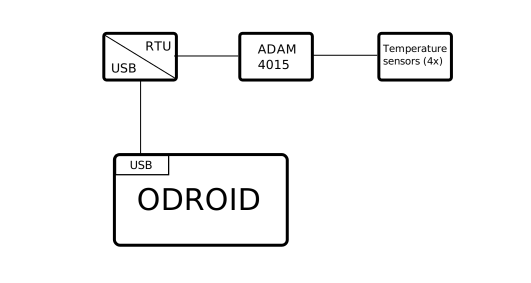
\includegraphics[width=0.6\textwidth]{images/ODROID_temperature_sensors.pdf}
      \caption{The connection of the weather station}\label{fig:temperature_sensors_connection}
\end{figure}

\subsubsection{Casting and scaling of temperature values}
Temperatures received from the ADAM-4015 module are encoded as a \verb|uint16_t|, but it was unknown how the module was programmed so it was yet to be determined what this value represents. To overcome this issue, The ``AdamApax .NET Utility'' \cite{AdamApax} was installed to investigate the settings that the module was operating at. The settings that were found can be seen in \Cref{fig:ADAM_-50-150}.\\

\begin{figure}[!ht]
  \centering
    \includegraphics[width=0.75\textwidth]{images/ADAM_-50-150.png}
      \caption{Settings of the ADAM-4015 Data Aquisition Module. Input range (top) shows the temperature range of -50\degree C to 150\degree C. The fourth connection shows the value that is used (23823), other sensors are not connected.}\label{fig:ADAM_-50-150}
\end{figure}

It was likely that the \verb|uint16_t| values could be cast to \verb|int|, and then be scaled between -50\degree C and 150\degree C. This would result in a temperature of $\frac{23823}{2^{16}-1} \cdot 200-50 = 22.70$\degree C. To confirm this, the settings were changed to output between -200\degree C and 200\degree C. The results can be found in \Cref{fig:ADAM_-200-200}.\\

\begin{figure}[!ht]
  \centering
    \includegraphics[width=0.75\textwidth]{images/ADAM_-200-200.png}
      \caption{Alternative settings of the ADAM-4015 Data Aquisition Module. Input range (top) shows the temperature range of -200\degree C to 200\degree C. The fourth connection shows the value that is used (36491), other sensors are not connected.}\label{fig:ADAM_-200-200}
\end{figure}

This capture was done close after the image in \Cref{fig:ADAM_-50-150} and results in a temperature of $\frac{36491}{2^{16}-1} \cdot 400-200 = 22.73$\degree C, which is similar enough to the previous calculation to conclude that this calculation is indeed correct.\\

The temperature values are therefore cast using the function found in Script \ref{castTempData}, after which they are scaled using the loop found in Script \ref{scaleTempData}.

\scriptsize
\begin{lstlisting}[language=C,caption={Function used to cast temperature data},label={castTempData}]
double* CastTempData(uint16_t *temperatures){

    //Cast the uint16_t array with temperatures to double
    double *double_temperatures;
    double_temperatures = (double *) calloc(NB_SENSORS, sizeof(double));

    int i;
    for(i = 0; i < NB_SENSORS; i++){
        double_temperatures[i] =(double)((int)((int16_t)temperatures[i]));
    }

    return double_temperatures;
}
\end{lstlisting}
\normalsize

\scriptsize
\begin{lstlisting}[language=C,caption={Function used to scale temperature data},label={scaleTempData}]
for(i = 0; i < NB_SENSORS; i++){
    double tmp = cast_temperatures[i]/65535*200-50; //scale linearly between -50 and 150 degrees
    scaled_temperatures[i] = roundf(tmp*100)/100; //round on two decimals
}
\end{lstlisting}
\normalsize

\subsubsection{Hotswap}
Due to the fact that the ADAM module gives values for ports that are available but not connected (65535) it is possible to implement a hotswap functionality to the temperature sensors. This means that it is possible to remove or add temperature sensors while the system is operational. The value of 65535 corresponds to 150\degree C and is not considered a realistic value for solar panel temperatures. This value will be sent to the server but will not be logged. It will be discarded instead. Whenever a sensor is added, however, this value will change and the server will know that a temperature sensor was added. Similarly, it will know when a sensor was disconnected by checking if the temperature value equals 150\degree C.

\subsubsection{Robustness}
A couple of checks are done in \verb|readTemperatureSensors| to ensure that the system can run 24/7 \ref{eis:2.3}. This is done by returning zero whenever a check fails (for example, a failed connection). The function that handles the data (see Script \ref{sec:code_overview}) will then check if a zero was returned. Whenever this happens, it will bypass updating the local display and the sending of data to the server.\\

The function will first check if a connection can be established to the ADAM module, this is done similar to the check in \verb|readWeatherStation| (see Script \ref{check_modbus_connection}). After reading the registers containing the temperature data, the function will check if all registers were read using the code found in Script \ref{check_temp_data_size}.

\scriptsize
\begin{lstlisting}[language=C,caption={Checking if the received data corresponds to the amount of requested registers},label={check_temp_data_size}]
if(rc!=NB_SENSORS){
	printf("FAILED (rc=%d) \n",rc);
	modbus_close(ctx);
	modbus_free(ctx);
	return 0;
}
\end{lstlisting}
\normalsize

	\subsection{Chargers}\label{sec:chargers}
\subsubsection{Controlling the chargers}
One of the main functionalities of the ODROID is to turn on the chargers if a user wants to charge an e-bike \ref{eis:1.6}. Turning on the chargers is done using a relais that is controlled by the ODROID. The relais can be turned on or off by using a signal from a GPIO pin.\\

At this moment the physical chargers that will be used in the charging station are not developed enough to be used for test purposes, hence another way to test the C-code must be designed. An easy way to check if the GPIO pins are turning the chargers on or off is by using LEDs that are connected to the GPIO pins. However, it is not desired to draw current for the LEDs directly from the GPIO pins. Since the driving current limit for the GPIO pins is 2-4 mA (not every pin has the same current limit) \cite{odroid_currentlimit}, it is neccesary to use an external driver for the LEDs. The easiest way of driving a LED is by using a voltage controlled switch. The voltage from the GPIO pins then determines whether the switch is open or closed. In electronic components, such a voltage controlled switch can be made by using a transistor \cite{switch_transistor}. To behave as a closed switch the transistor must be in saturation, because then the collector to emitter resistance is very low and the transistor almost acts as a short circuit. For the transistor to behave as an open switch, it must be in cutoff mode.\\

\begin{figure}[!ht]
  \centering
    \includegraphics[scale=1.5]{images/led_driver_schem.pdf}
      \caption{Circuit used to drive the LED. Made using Fritzing \cite{fritzing}}\label{fig:leddriver}
\end{figure}

The transistor used for this circuit is a bipolar P2N2222A NPN transistor. This is a general purpose transistor that can be used for power amplification as well as switching applications requiring collector currents up to 500mA \cite{p2n2222a}.\\

\Cref{fig:leddriver} shows the circuit that is used. Resistor Rc is chosen such that the current through the LED is limited if the LED turns on, hence a maximum current of $\frac{5}{330}=15mA$ can be drawn from the source. However, since there is also a voltage drop over the LED this current will be much smaller and well below the current limit for this LED.\\

In order to act as a buffer, the circuit should draw as less current as possible from the GPIO pins of the ODROID. This is achieved by choosing a very high base resistance Rb. However, a base resistance that is too high results in malfunctioning of the transistor because not enough current is fed into the base. 

When the transistor is in saturation the base voltage is about 0.7V thus the base current is about $\frac{3.3-0.7}{Rb}$. To achieve a base current of 0.1mA a resistance Rb of 26k$\Omega$ is needed. However, after a test this resistance was found out to be too large. A smaller resistor of 10k$\Omega$ solved this problem.\\

The circuit shown in \Cref{fig:leddriver} is built six times and then connected to the six GPIO pins of the ODROID that are used to control the chargers \ref{eis:3.4}.\\

\subsubsection{Detection of the charging cable}
To increase the level of safety for the users the chargers should not be turned on when there is nothing connected to them. Therefore a charging cable detection system is designed. For each cable one additional GPIO pin is needed (of course the ground pin on the ODROID is also needed). In case of a connected charging cable, this GPIO pin is shorted to ground (inside the charging cable) and thus a logic 0 is set to this pin. In the other case (no connected charging cable), the pins keep floating. However, the ODROID can be programmed such that it internally connects a pull-up resistor to the pin. Now a logic 1 is detected whenever no charging cable is detected. Within the C-code this can be detected by using the \verb|digitalRead()| and \verb|pullUpDnControl()| functions.\\

\begin{figure}[!ht]
  \centering
    \includegraphics[scale=1.7]{images/cable_detection_schem.pdf}
      \caption{Circuit used to detect the connected cable using a GPIO pin \cite{fritzing}}\label{fig:cable_detect}
\end{figure}

\Cref{fig:cable_detect} depicts the circuit that is used for this purpose. Since there are no available charging cables yet, a switch was used in this circuit to simulate the behaviour of the cable. It was also chosen to include a 2.7k$\Omega$ resistor in series with the switch. As a testing circuit some precautions have to be taken to ensure that nothing can be damaged as a result of short circuits. This also results in a choice for the value of resistor R2. The lowest current limit of all GPIO pins is 2mA. Together with a maximum voltage of 5V on one of the pins, a 2mA current limit means that R2 must be at least 2.5k$\Omega$.\\

But R2 may limit the short circuit current, it also influences the voltage at the pin. The voltage division on R1 and R2 makes that it is no longer possible to obtain 0V at the GPIO pin. With the switch in closed state, the voltage is $\frac{R2}{R1+R2}\cdot 3.3 = \frac{2.7}{62.7}\cdot 3.3=0.14V$. Altough this voltage is not zero, it is nevertheless low enough for the ODROID to detect it as a logic low or 0. With the switch in opened state, this voltage division does not occur and will thus not impose problems with respect to the input voltage.\\

\subsubsection{Control mechanism for the chargers}\label{sec:charger_control}
When a reservation is made in the end-user interface the state of the charger in the database is set to 1. Using the C-code on the ODROID this data can be retrieved from the server. When calling the function \verb|getChargerState()| an array of length 6 is returned, containing the server state of all chargers. As explained in \Cref{sec:code_overview} the chargers are set every 1.5 seconds using the function \verb|setChargers()|.\\ 

For the design of this control mechanism some additional functionalities were set up to improve user-friendliness and safety. These are:
\begin{itemize}
\item When a reservation is made on the website, but the owner of the e-bike does not show up within 60 seconds, the charging point is released. This ensures that it is not possible to claim charging points without actually charging.
\item The chargers will only be switched on when a cable is connected for more than 6 seconds.
\item In case of a cable that is being disconnected during charging, the chargers will turn off, but remain reserved for 15 seconds. A cable that is plugged out accidentally can now be replaced without having to login again.
\item The admin-dashboard must be able to turn off a charger, even when a vehicle is connected.\\
\end{itemize}

\begin{figure}[!ht]
  \centering
    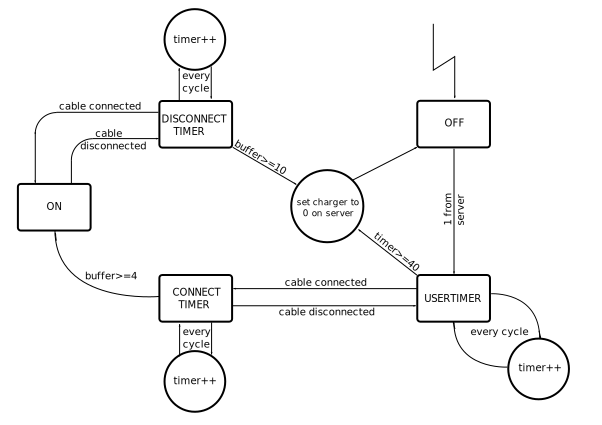
\includegraphics[width=\textwidth]{images/Charger_Control.pdf}
      \caption{FSM to control the chargers}\label{fig:fsm}
\end{figure}

To implement these functionalities, it can be seen that three different timers are needed and thus some form of memory to store these timers. Moreover, the chargers must refresh or reset every time the variable \verb|j| from \Cref{fig:code_overview} is incremented (every 1.5s). All these functionalities can now conveniently be combined in a Finite State Machine (FSM) that uses a change in \verb|j| as the clock. \Cref{fig:fsm} depicts the finite state machnine that was designed for this purpose.\\

The diagram starts in the reset state, which is the OFF state. It only leaves this state when a reservation is made and the server says that a charger must be turned on. In that case the finite state machine goes into the USERTIMER state. Here it waits until a cable is connected. When no charging cable is connected within 60 seconds, the FSM goes back to the OFF state and sends a message to the server that the charger can be freed for other users. In the other case (charging cable is connected within 60 seconds), the FSM goes to the CONNECTTIMER state. Here it waits 6 seconds until it moves on to the ON state where the chargers are switched on. However, if the cable is disconnected within these 6 seconds, the FSM returns to the USERTIMER state. Now the cable must be plugged in for another 6 seconds before the chargers are switched on.\\

Now suppose the e-bike is being charged and the finite state machine is in the ON state and the charging cable is disconnected. This can be due to two reasons: the e-bike is charged and leaves, or the e-bike is accidentally unplugged. Both cases will make the FSM move to the DISCONNECTTIMER state where the charger is turned off. If the cable is reconnected within 15 seconds, the FSM moves back to the ON state and the charger is turned back on again. On the other hand, after 15 seconds of no reconnection, the charger is left off and the FSM moves to the OFF state.\\

Finally, if the FSM moves to a next state, the timer of the corresponding state that is left, is reset. All three timers are reset when a charger is turned off on the admin-dashboard. The FSM then always moves to the OFF state.\\

To obtain a Moore machine, the output signals must only depend on the current state. Hence the chargers are turned on only in the ON state, whereas in all other states, the chargers are off. Using the C library \textit{WiringPi} \cite{WiringPi} it is possible to easily write a logic 0 or 1 to the GPIO pins and effectively turn the chargers on or off \cite{wiringpi_functions}. The GPIO \textit{WiringPi} pin numbers used for this purpose are 6, 10, 11, 12, 13 and 14 for the chargers and 21, 22, 23, 24, 26 and 27 for the cable detection \cite{odroid_specs}. Each of the six chargers is controlled by an FSM and hence 6 FSMs are neccessary to control all chargers. It is chosen to implement this by using a \verb|for|-loop.

\subsubsection{Internet failure failsafe}
A failsafe was implemented which ensures that e-bikes are not connected for too long when internet is unavailable. This is important because the station cannot be monitored online during an internet outage. A timer was made that keeps track of how long the internet has been down for. It was decided that all chargers should be turned off whenever the internet is out for more than 2 hours. This time was chosen because it enables the station to finish the charging of any e-bike that is already connected, while also limiting potential risks of an unmonitored system.\\

\scriptsize
	\lstinputlisting [language=C,caption=Internet failure failsafe,label=script:internet_failure_failsafe] {code/internet_failure_failsafe.c}
\normalsize

The implementation of this failsafe can be found in Script \ref{script:internet_failure_failsafe}. In this function, the first \verb|if| statement checks if the data fetch was successful. In this statement, the \verb|noConnectionTimer| is set to zero. The \verb|else|-statement is executed whenever connection was not successful. In this part, the \verb|noConnectionTimer| is incremented (or set to one if the system just booted with no connection). The timer value is then checked if it is larger than $2\cdot60\cdot60/1.5=4800$ (one poll every 1.5 seconds), and the GPIO pins are set to low if it is. Note that the \verb|for|-statements in the case of no connection manage the charger GPIOs and the FSM states as described in \Cref{sec:charger_control} (omitted for the sake of simplicity).
	\subsection{Local display}\label{sec:display}
\subsubsection{Display data file}
To display data on a local webpage \ref{eis:1.4} \ref{eis:1.5}, it was decided that it would be the most convenient to write data to a text file, which would then be read by a script that controls the webpage. Because this read script would most likely be a JavaScript file, it was thought that the text file should be of the .json format. The code that is used to print this .json file can be found in Script \ref{print_json}.

\scriptsize
\begin{lstlisting}[language=C,caption={Writing a .json file for the local webpage},label={print_json}]
FILE *f = fopen("localDisplayData.json", "w");
if (f == NULL){
	printf("Error opening file!\n");
} else {
	fprintf(f, "{");
	fprintf(f, "\"temperature\": %f,\n", weatherFinalValues[5]);
	fprintf(f, "\"wind-chill\": %f,\n", weatherFinalValues[6]);
	fprintf(f, "\"humidity\": %f,\n", weatherFinalValues[7]);
	fprintf(f, "\"wind speed\": %f,\n", weatherFinalValues[8]);
	fprintf(f, "\"radiation\": %f,\n", weatherFinalValues[9]);
	fprintf(f, "\"air pressure\": %f,\n", weatherFinalValues[10]);
	fprintf(f, "\"wind direction\": %f\n", weatherFinalValues[11]);
	fprintf(f, "}");
	fclose(f);
}
\end{lstlisting}
\normalsize

\subsubsection{Testing the local webpage}
A simple webpage was made to ensure that running the local webpage by reading the text file is possible. A problem could arise, for example, because the two programs are both accessing the same file.\\

The JavaScript file can be found in Script \ref{script:JavaScript_test}. The script makes use of \textit{Ajax} \cite{jquery} to asynchronously refresh the webpage, so it will refresh the data without refreshing the entire webpage. It will read the \verb|localDisplayData.json| file every second (line 11) and will write this information to an HTML file (see Script \ref{script:HTML_test}). This writing is done in line 4 to 6 of Script \ref{script:JavaScript_test}.\\

\scriptsize
	\lstinputlisting [language=Java,caption=Test code for reading the .json file,label=script:JavaScript_test] {code/LocalDisplay.js}
	\lstinputlisting [language=HTML,caption=HTML file for displaying the data of the .json file,label=script:HTML_test] {code/LocalDisplayTest.html}
\normalsize

\subsubsection{WebGL}
The webpage, designed by another team within project SUNRISE, makes use of WebGL to display the information generated by the ODROID. A guide made by Hardkernel was used to install WebGL on the ODROID \cite{WebGL_guide}, after which a tip on their forum was used to enable WebGL in Chromium \cite{WebGL_forum}.\\

At first, these solutions, including many others, were unable to get WebGL running on the ODROID, eventhough the ODROID should be able to run WebGL. A lot of time was spent trying to fix this, after which it was decided that a good option might be to simply use a fresh install of the operating system. This was done by using a new ODROID C1+ (so the previous ODROID could still be used as a backup). This device was able to run WebGL after using the earlier mentioned sources. It is unclear why this was the case, but it is thought that the previous ODROID was either partly broken or had some setting disabled by a previous developer.\\

During the configuration of the new ODROID, it was decided that it would be convenient for future development to make an instruction file containing all elements that need to be installed and configured to be able to run all the systems. This instruction can be found in Appendix \ref{app:setup_manual}.

\subsubsection{Remote desktop}
The ODROID should be accessable remotely because it is not easily reachable when it is integrated in the charging station \ref{eis:2.1}. There are two elements required for this to work: a VPN connection to the router in the station and a remote desktop client. For the VPN connection, the OpenVPN  client \cite{openvpn} was used. This required VPN files that can be downloaded from the router.\\

During the first setup of the VPN this solution did not work. It took some time to figure out that the downloaded files were not configured correctly and needed to be edited before they could be used. A more detailed description can be found in the setup manual (see Appendix \ref{app:setup_manual}).\\

Finally, ``Remote Desktop Connection'' (installed default on Windows) was used to connect to the ODROID. For the ODROID to facilitate this connection, it needs a couple of packages. This too is described in detail in the setup manual (see Appendix \ref{app:setup_manual}).
	\subsection{Bash}\label{sec:bash}
For the system to correctly function, a couple of scripts had to be designed in Bash. These scripts take part in ensuring that the system remains functioning \ref{eis:2.3} or is able to recover after a power failure \ref{eis:2.2}. All scripts are booted on startup of the desktop using the \textit{Upstart} \cite{upstart} package. A \verb|README| file was made on the desktop of the ODROID to describe the scripts and holds information about how to turn them off (See Appendix \ref{app:bash_readme}). This was done to ensure easy future use.

\subsubsection{Xvnc killer}
One of the first observations that was done when the remote desktop functionality was working, was that the ODROID was significantly slower whenever someone connected. This is as expected, because the ODROID simply has more information to process. However, this issue remained even when all remote desktops were closed. It became an even greater issue when the ODROID could not handle all the processing anymore, after which it would completely freeze for up to an hour.\\

It was later discovered that a program called \verb|Xvnc| would boot whenever a remote desktop connected, and would not shut down when the user disconnected. A Bash script was therefore made that would count the number of open \verb|Xvnc| processes, and that would kill the oldest if it exceeded a certain amount (See Script \ref{script:xvnc}). This was done in a similar way for a processes called \verb|ssh-agent|, which booted in conjuction with \verb|Xvnc|. \verb|Xvnc_killer.sh| is booted on startup using an \verb|Upstart| file (See Appendix \ref{app:xvnc_killer_conf}).

\scriptsize
	\lstinputlisting [language=Bash,caption=Xvnc\_killer.sh,label=script:xvnc] {code/Xvnc_killer.sh}
\normalsize

The script uses \verb|ps aux| to list all the processes, \verb|grep| to search for a specific process, \verb|grep -v| \verb|'<defunct>'| to remove zombies (if a process did not shut down correctly it remains in the processes list without using any memory) and \verb|-gt| to check if the search returns a value greater than 4. If there are more than 3 clients connected (the search function also finds itself as a process), it will kill the oldest running client. This is done by sorting by the time the process booted by using \verb|sort -n -k 9| (this will sort by the 9th column: start time), picking the process ID column by using \verb|awk '{print $2}'| (this prints column 2: process IDs) and then picking the oldest process using \verb|head -1|. The \verb|kill| command kills the process that has this ID. Finally, the script sleeps for a minute, after which it repeats the cycle.

\subsubsection{Browser booter}
The browser booter was designed to automatically boot a browser for the local display \ref{eis:1.4}. The display should only show the local webpage, nothing else. This implies that it has to boot full-screen and that it should not display a scroll bar nor a mouse. An \textit{Upstart} file was made to boot the Chromium browser (See Appendix \ref{app:browser_boot}). This boot uses two flags: \verb|--use-gl=egl| to enable WebGL features used in the local webpage and \verb|--kiosk| to boot full-screen. A bash script was made to start the \textit{Unclutter} \cite{unclutter} package on startup, which was set to hide the mouse after 5 seconds of inactivity (see Appendix \ref{app:hide_mouse} and \ref{app:hide_mouse_conf}). 

\subsubsection{C-code booter}
The C-code booter was made to boot the C-code on startup (see Appendix \ref{app:odroid_boot} and \ref{app:odroid_boot_conf}). This can be useful when the system has been troubled by a powercut \ref{eis:2.2}. The booter will also check if the program remains running, and it will reboot whenever it finds that it is not. Several flags in the command will ensure that the terminal does open (using \verb|-hold|), but not in front of the browser (using \verb|-iconic|). The \verb|su| command is used because the code requires a SuperUser (because of the control of GPIO pins).
		\clearpage    	
    \section{Results}\label{sec:results}
% Testen van het weerstation (ventilator, zon, etc.)
% Victron verifiëren via CCGX, vermogens van de twee multiplus systemen
% GPIO's
% Robuustheidstest (random dingen uitpluggen, langer laten draaien, etc.)
% valgrind
% manual in appendix noemen

\subsection{Weather station}
To verify correct functionality of both the weather station and the communication with the ODROID, a simple test setup was conducted to test all the used sensors. Most sensors could be read at any time (temperature, humidity, air pressure). However, both the radiation sensor and wind sensors would register zero because there was not enough light and wind to trigger these sensors. The weather station was set up at the window on a bright day to test the radiation sensor, and a fan was placed to check if the wind was received correctly. During these tests, all sensor values were correctly read and sent to the server. This confirmed the functionality of both the weather station and the communication with the server.

\subsection{Victron system}\label{sec:victron_results}
For reading the registers of the Victron system the Modbus libraries are used. By printing the read values to the screen it was easily verified that the ODROID was able to read the Victron system.\\

To determine what the registers with respect to the power represent, a load was connected to the system. An easy way to do this is by connecting a large power resistor to the system. The power dissipated in this resistor was recognized as DC power on the Victron system. \\

%However, it was not possible to read this register using the  ODROID.\\
Some 230V sockets are also connected to the Victron system. The ODROID, router and display are connected to these sockets. By switching the display on, an increase in AC power was detected in one of the MultiPlus slaves (slave ID 0). The other MultiPlus slave, however, did not register it, so it was clear that although they are the same physical device, they do register different information.\\

To find out what they are measuring, the systems were both monitored for roughly a day. The results of input power can be found in \Cref{fig:MultiPlus_inputs}. The peak of roughly 1.8kW is the moment that the Victron system starts charging the batteries with energy from the grid.\\

\begin{figure}
\centering
\begin{subfigure}{.5\textwidth}
  \centering
  \includegraphics[width=.95\linewidth]{images/Input_power_30W.png}
  \caption{MultiPlus on slave ID 0}
  \label{fig:MultiPlus_input_30W}
\end{subfigure}%
\begin{subfigure}{.5\textwidth}
  \centering
  \includegraphics[width=.95\linewidth]{images/Input_power_70W.png}
  \caption{MultiPlus on slave ID 246}
  \label{fig:MultiPlus_input_70W}
\end{subfigure}
\caption{Input power of the MultiPlus slaves}
\label{fig:MultiPlus_inputs}
\end{figure}

At first, these graphs look identical. However, closer inspection reveals that the device at slave ID 0 has a standby power of 30W, and the other device has a standby power of 70W. There are also minor differences in the peak during charging. Similar results are found for the output powers.\\

Concluding, it is thought that MultiPlus devices both monitor the AC power regarding the batteries. External AC connections (e.g. router, local screen, etc.) are found in the MultiPlus device with slave ID 0, and all internal AC power (all the Victron devices) are monitored by the MultiPlus device with slave ID 246. The last guess is mainly based on the fact that the 70W standby does not change when anything is connected, and 70W is in the order of power usage of the Victron systems.\\

Another important result is that it is not possible to read all the registers that are mentioned in the register list. Most of these unreadable registers are a result of devices that are not connected due to the modularity of the Victron system. Moreover, it was not possible to read the state of health of the batteries on register address 304, despite the fact that there is a battery management system inside. It is unclear why this register cannot be read, but it is likely that it is simply not supported by the batteries that are used.

\subsection{Chargers}
The chargers are tested in a conceptual way by controlling the LEDs connected to the GPIO pins. Beforehand it is of course necessary to test the driver that is used for the LED as shown in \Cref{fig:leddriver}. During the test a 5V and 3.3V supply were used to deliver the energy.\\

First, the value of the highest possible Rb was determined. When using a 22k$\Omega$ resistance the transistor did not function as desired, hence a smaller resistor needed to be selected. A 10k$\Omega$ resistance Rb was enough to ensure that sufficient current could enter the base of the transistor. However, the current through the base is inversely proportional to the resistance Rb. This is a result of the constant voltage drop of about 0.7V over the base-emitter junction. A smaller Rb thus results in a higher base current and hence an increased current drawn from the GPIO pin.\\

When the transistor is in saturation, a voltage of about 0.69V was measured at the base terminal. The voltage at the collector terminal was about 0.073V. Now it can be concluded that the transistor is indeed in saturation. At the base, the voltage is higher than at the collector and the emitter. Using the fact that the P2N2222A is an NPN transistor it means that both the base-emitter junction and the base-collector junction are forward biased. Using these measurements and the value of Rb the base current is $\frac{3.3-0.69}{10k}=0.26mA=260\mu A$.\\

A voltage of 1.69V was measured over Rc; hence the current through the LED equals 5.1mA which is enough to make the LED clearly visible. By using the state of the chargers fetched from the server, the GPIO pins were set to a logic 0 or 1. A change in the state of a charger in the database was indicated on the LEDs in less than 1.5 seconds.\\

The FSM controlling the chargers was tested by connecting both the LED array (described above) and the switch described in \Cref{fig:cable_detect}. All the state changes were tested on their functionality (by printing all current states) as well as their timing (counting the number of cycles until a state change). This resulted in no significant problems, however it was evident that not all functionality was present. The main issue was that the charger would not respond to the administrator turning off a charger. This was solved by making an \verb|if|-statement that sets the local charger state to OFF for all chargers that are set to 0 on the server. This force-statement resets all timers used in any of the states.

\subsection{Solar panel temperature sensors}
The temperature probes were easily tested by reading the registers from the ADAM module to which they are connected. Using the Modbus routines to read registers data was obtained. During the test, only one temperature sensor was connected (there are 5 more slots available to connect temperature sensors). From the registers that were not connected to a temperature sensor, the value $2^{16}-1=65535$ was returned, which means it is unconnected but functioning. Register 4, to which a sensor was connected, returned a value between $0$ and $2^{16}-1$. Using the mapping as described in \Cref{sec:temp_sensors} this value was mapped to a temperature, which indeed corresponded to the current room temperature.

\subsection{Local Display}
The file that contains the data for the local display is correctly generated every 15 seconds by the display function. The webpage that is going to be displayed in the actual charging station is yet to be finished by another team in project SUNRISE, thus the actual implementation of reading this file is yet to be finalized. However, all other necessary precautions have been taken regarding this webpage: the ability to run WebGL and the ability to automatically boot all display programs (see \Cref{sec:bash_results}). A small script was also written to test the reading of the file, and the data was displayed and refreshed without any issues (see \Cref{fig:test_display}).

\begin{figure}[!ht]
  \centering
    \includegraphics[width=0.15\textwidth]{images/test_display.png}
      \caption{Output of the test webpage}\label{fig:test_display}
\end{figure}

\subsection{Bash}\label{sec:bash_results}
The bash scripts all function as designed. The scripts can boot the browser on startup, boot and reboot the C-code, ensure there are not too many remote desktops connected and hide the mouse so it does not display on the local display.

\subsection{General testing}
\subsubsection{Memory leaks}
Although the C-code was written with the utmost care, chances are that not all memory allocations are freed. Because the code is running 24/7, any memory leaks would sooner or later become an issue for the system. It was therefore necessary to ensure no memory leaks were created by the code.\\

A Linux tool called ``Valgrind'' \cite{valgrind} was used to check the code of any memory leaks. Valgrind has a tool specifically designed for this: memcheck. Two memory leaks were found by this tool, both caused during casting of data. The problem was that a variable that would contain the result of the casts function had memory allocated. However, the same memory allocation was done within the cast function. The earlier mentioned variable would be overwritten by the data of the cast function, causing it to lose the location of the memory that was allocated to it. A memory leak was mentioned by Valgrind, and some manual searching of the code led to the core of the problem.\\

In later stages of the design, it was decided that memory allocations should be removed alltogether (if possible). This is further explained in \Cref{sec:malloc}.

\subsubsection{Long term tests}
The ability of the code to run for a longer time is a very important aspect to test. Multiple tests were conducted in which the code would run overnight by using Valgrind. During these test all available functionality of the code was used (reading the devices, controlling the GPIO pins and sending and receiving data from the server). Both tests resulted in a failure of the code. The database showed that data had been received up until 3 a.m. and then nothing more was received. The terminal window in which the program was running showed that wrong data was received on the ODROID about the state of the chargers. Only zeroes and ones should be received, however some random values were received which caused the program to crash. This is probably a result of a kind of reset that is done every night on the server of TU Delft. The server code did return a null pointer when no data was received, but this result was not checked and was therefore still written to the pins. This was probably random memory data, which finally crashed the program.\\

In the end, roughly 6 long-term tests were conducted, ranging between 24 and 96 hours. The duration of a full cycle (\Cref{fig:code_overview}) was not very constant, but it did not deviate more than about 15 seconds from the 5 or 10 minute cycle. This will not be a major issue since this deviation did not accumulate after several cycles.\\

\subsubsection{Robustness tests}\label{sec:robustness_tests}
To guarantee robustness, it was important to unplug and replug all ODROID connections multiple times. This reveiled some minor bugs regarding server connectivity, but ultimately resulted in sturdy code that will simply reconnect whenever a device becomes available again.\\

A more interesting result occurred when unplugging both Modbus RTU connections (temperature probes and weather station). This sometimes resulted in the devices not being found after reconnecting. It was soon noticed that the order in which the devices are connected is important. Due to limited development time, it was not considered important enough to dynamically allocate these USB connections to make the ODROID independent of connection order (if at all possible). Until that time, the USB of the temperature sensors should be plugged in before the weather station. 
        \clearpage     
 	\section{Discussion}\label{sec:discussion}
\subsection{Desynchronization}
Although the loops described in \Cref{sec:code_overview} take only a couple of milliseconds to execute, it is technically possible that they take more than 1.5 seconds to complete. For example, when \verb|j| equals 400, both \verb|weatherDisplay()| and \verb|functionVictronData()| have to be executed. This could potentially cause a small desynchronization.\\

To overcome this, functions could be seperated in smaller chunks. For example, splitting the three Victron functions, or even seperating fetching and sending of data. This will decrease the chance of a function taking more than 1.5 seconds to execute. Another solution could be the use of threads, so whenever a thread is unable to finish within 1.5 seconds, it will simply run parallel to the main function. With this implementation one should be careful not to have a weather station function and a temperature probe function fetching data at the same time, because the ADAM-4015 module cannot handle two parallel requests.\\

This potential issue is, however, not likely to occur in practice and will make the code unnecessary complex. Functions are simply executed too fast to cause any desynchronization (e.g. fetching and sending Victron data, weather data and charger data takes only 0.23 seconds at most), and even if it should happen, there is only a desynchronization in the order of a few seconds, which is not an issue. The sleep function (that is used to halt the program when 1.5 seconds have not yet passed) has also been secured by not executing whenever a negative amount of seconds is remaining (when it is taking more than 1.5 seconds), because it will run indefinately if a negative amount is entered.\\

Although the problem mentioned above has not occurred during testing, a cycle would still take longer than expected (10 seconds longer every 10 minutes). This desynchronization is caused by the code between calculating the remaining time until 1.5 seconds and sleeping (see Script \ref{desync}). Line 3 and 6 therefore take roughly $\frac{5}{5*60}=25$ms to execute. This issue can be solved by decreasing \verb|loop_time| by 25ms. However, because this is not really an issue (and it is not really predictable), it was decided that this correction was unnecessary complex, thus it was not implemented.

\scriptsize
\begin{lstlisting}[language=C,caption={A cause of small desynchronization},label={desync}]
	diff = clock()-start; //calculate remaining time

	printf("the time taken was %f \n",((float)diff/CLOCKS_PER_SEC));

    //Make sure the cycles do not take less than 1.5 seconds
	n = (int)((loop_time - ((double)diff)/CLOCKS_PER_SEC) * 1000000);
	if (n>0) usleep(n); /*pause before next iteration*/
\end{lstlisting}
\normalsize

\subsection{Memory allocation}\label{sec:malloc}
\Cref{fig:code_overview} shows that the program is built on an endless loop in which data is fetched and sent to the server. Since the data is stored in arrays it might be tempting to use dynamic memory allocation by using \verb|malloc| or \verb|calloc|. However, the program must run 24/7 \ref{eis:2.3} and therefore memory leaks are not permitted. As dynamic memory allocation is a major cause of memory leaks, it was chosen to use dynamic memory allocation only if it was absolutely necessary. Regarding the flexibility and optimal usage of memory resources, it may be an advantage to use \verb|malloc| or \verb|calloc|. On the other hand, in larger programs a common mistake is to forget the use of \verb|free()| to empty the used memory. Even more so when a variable is allocated and freed in different functions.\\

In the C-code it is therefore chosen not to use dynamic memory allocation. As a result, no \verb|free()| is necessary and memory leaks are avoided. All arrays containing the station data are declared only once. To be able to use the arrays in multiple C-files, the arrays are defined \verb|extern|. Unnecessarily passing the arrays as a function argument is prevented this way. Defining the length of the arrays is now done during compile time and therefore the length of the arrays cannot be a variable but must be a constant. This constant is chosen such that it can contain the maximum amount of registers that can be read in one request. For example, the maximum amount of registers that can be read from the Victron system using a single function call of \verb|readVictron()| is 46. The length of the predefined array to store is registers is thus 46. 

\subsection{Temperature sensor polling failure}\label{sec:temperature_sensor_failure}
Although the ODROID can fetch data from the solar panel temperature probes through the ADAM-4015 module, it regularly fails in doing so. A failure in polling the temperature sensors happens in roughly $\frac{1}{3}$rd of the fetches. This problem is unlikely to be caused by the ADAM module, because this can handle a polling rate of 12 per second \cite{adam_polling}. It is unclear if there is a maximum polling rate to the temperature probes, but these probes are most likely analogue and therefore not bound to a maximum polling rate.\\

It is therefore unclear what causes these frequent failures. The functionality is present, however, so data can be read, but it should be inspected more closely in future development if more data is desired.
%polling failures
 		\clearpage
  	\section{Conclusions}\label{sec:conclusions}
\subsection{General conclusion}
The goal of the overall project was to design software packages and an intuitive user-interface for an e-bike charging station. Users can make a reservation in the user-interface after which they can charge their e-bike in the charging station. The main focus in the design process described in the sections above was the low-level design of data acquisition and control of the chargers using an ODROID minicomputer.\\

All targets with respect to the data acquisition were reached: the C-program on the ODROID is able to read all data generated by the power electronics, weather station and temperature sensors. Using the GPIO pins from the ODROID the relais can be controlled, which turn on/off the chargers. This concept was succesfully tested using LEDs since the chargers were not finished yet. Furthermore, a charger control Finite State Machine was designed and tested. This controller has buffers so the charger state does not immediately change when a cable is (dis)connected (for example, plugging the cable in badly could cause it to turn on and off immediately), as well as a timer between logging in on the server and plugging in. At this moment it is not yet possible to control the local display which will be mounted in the charging station, because there is no webpage yet to control. A conceptual design for the control mechanism is available though, including the working WebGL on the ODROID for the graphical elements of the webpage.\\

During tests of multiple days the C-code was succesful with respect to robustness and memory leaks. Moreover, additional Bash scripts were written to support the functionality of the code. For example, a script to solve memory leaks caused by the remote desktop was written, as well as a script to immediately start certain programs on the ODROID after a reboot (a full-screen browser and the C-code). Finally, an installation and configuration manual was made. Using this manual it is possible set up a new ODROID using some easy steps. After performing these steps the C-code should be able to run on the ODROID.\\

 	\subsection{Future work and recommendations}\label{sec:future}
As a low-level part of the charging station the ODROID must have solid software packages. To further improve the functionality and stability of this software some general ideas are given that can be elaborated in the future.\\

%An important feature of the charging station is the detection of a charging cable that is unplugged. If a charging cable accidentally is pulled out or an e-bike is removed, the chargers must turn off. Another GPIO pin from the ODROID can be used, together with some circuitry, to test whether a charging cable is connected or not. Using this feature it now also becomes possible to only turn on the chargers once an e-bike is connected, instead of directly turning it on when a reservation is made. At this moment, this feature is not yet available. However, some testing was done with this concept. \\

%To achieve a higher level of safety the chargers must be turned off when the program happens to fail. For example, if a logic high is written to a GPIO pin, and thus essentially a charger is turned on, the GPIO pin remains at a logic high when the program crashes. Of course such behavior is not desired, hence a separate program can be written that checks if the main program is running. It can then restart the main program such that the chargers are again controlled in a correct way.\\

As an additional feature for end-users, the battery voltage of their e-bikes could be displayed on the webpage. A sensor and all the neccesary circuitry can be developed in the future for this purpose. The C-code running on the ODROID also has to be adapted to read the sensor values and transfer the data to the server.\\

%When the internet connection fails it is important that the program still keeps running. However, since no data can be received from the server, no new e-bikes can be connected for charging. Turning off the chargers for e-bikes that were already charging is not desired and hence a solution must be found for this issue. If the charging cable detection is finished, this detection be used for this issue as well. For example, during a longer internet failure, the chargers can be set to charge for a maximum of a few hours and turn off when either the charging cable is disconnected or the time limit expires.\\

\Cref{fig:station_concept} shows that a local display will be mounted on the charging station. As a clearly visible device it is therefore important to have it running by the time the charging station is built. Currently, only the concept of the controlling mechanism is designed. The final implementation of the website together with the JavaScript and C-code still have to be designed and tested. Moreover, it is always possible to improve the information shown on the webpage and the design of the webpage itself.\\

During robustness tests (see \Cref{sec:robustness_tests}), it was discovered that the order in which the USB connections of the temperature probes and weather station were connected was of importance. This was due to the fact that the connection was established statically in the C-code. In future work, this could be allocated dynamically. By doing this, the connection order is no longer of importance, and the system will be more robust (for example during maintenance).\\

As described in \Cref{sec:temperature_sensor_failure}, polling the temperature sensors is quite known to fail. The code was designed to never cause the C-code to crash when this happens, however it does mean that data points are missing about a third of the time. If a more regular set of data is desired, more research has to be done to extract the issue that causes this problem.\\

As an addition to the existing concept of the charging station, a LED strip could be added to the exterior of the station (behind matte glass, for example). This could be controlled by the ODROID based on the input of several proximity sensors. The LED strip should be fed by an external power supply (since these require a lot more power than the GPIO pins can deliver), probably a 230V connection of the Victron system. One should keep an eye on the number of available GPIO pins if this were to be developed.

%Not sure about this one
%USB allocations (wordt nu statisch gedaan maar kan waarschijnlijk ook dynamisch)
 		\clearpage
    
%%%%%%%%%%%%%%%%%%%%%%%%%%%%%%%%%%%%%%%%%%%%%%%%%%%%%%%%%%%%%%%%%%%%%%
%							Bibliography
%%%%%%%%%%%%%%%%%%%%%%%%%%%%%%%%%%%%%%%%%%%%%%%%%%%%%%%%%%%%%%%%%%%%%%

%	\bibliographystyle{plain}
%	\bibliography{bibliography}

	\bibliographystyle{IEEEtran}
%	\nocite{*}
	\begingroup
	\raggedright
	\bibliography{bibliography}
	\endgroup

%%%%%%%%%%%%%%%%%%%%%%%%%%%%%%%%%%%%%%%%%%%%%%%%%%%%%%%%%%%%%%%%%%%%%%
%								Appendix
%%%%%%%%%%%%%%%%%%%%%%%%%%%%%%%%%%%%%%%%%%%%%%%%%%%%%%%%%%%%%%%%%%%%%%

	\clearpage
	\section*{Appendix}	
	\renewcommand\thesection{\Alph{section}}	
	\setcounter{section}{0}
		\section{Setup manual}\label{app:setup_manual}
\scriptsize
\lstinputlisting[language={},numbers=none]{code/ODROID-Instructions.txt}
\normalsize
		\section{Bash files}
\subsection{Startup Programs README}\label{app:bash_readme}
\scriptsize
\lstinputlisting[language={},numbers=none]{code/README_startup_programs.txt}
\normalsize

\subsection{Xvnc\_killer.sh}\label{app:xvnc_killer}
\scriptsize
	\lstinputlisting [language=Bash] {code/Xvnc_killer.sh}
\normalsize

\subsection{Xvnc\_killer.conf}\label{app:xvnc_killer_conf}
\scriptsize
	\lstinputlisting [language=Bash] {code/Xvnc_killer.conf}
\normalsize

\subsection{hide\_mouse.sh}\label{app:hide_mouse}
\scriptsize
	\lstinputlisting [language=Bash] {code/hide_mouse.sh}
\normalsize

\subsection{hide\_mouse.conf}\label{app:hide_mouse_conf}
\scriptsize
	\lstinputlisting [language=Bash] {code/hide_mouse.conf}
\normalsize

\subsection{browser\_boot.conf}\label{app:browser_boot}
\scriptsize
	\lstinputlisting [language=Bash] {code/browser_boot.conf}
\normalsize

\subsection{ODROID\_booter.sh}\label{app:odroid_boot}
\scriptsize
	\lstinputlisting [language=Bash] {code/ODROID_booter.sh}
\normalsize

\subsection{ODROID\_booter.conf}\label{app:odroid_boot_conf}
\scriptsize
	\lstinputlisting [language=Bash] {code/ODROID_booter.conf}
\normalsize

		
        
%%%%%%%%%%%%%%%%%%%%%%%%%%%%%%%%%%%%%%%%%%%%%%%%%%%%%%%%%%%%%%%%%%%%%%

\input{backpage}

\end{document}